\chapter{Regimes de Volatilidade e o Prêmio de Risco de Volatilidade do Bitcoin}
\label{chap:regimes}

\section{Motivação e Objetivo do Capítulo}
\label{sec:cap9_motivacao}

Os capítulos anteriores estabeleceram que o Prêmio de Risco de Volatilidade do Bitcoin
(BVRP) é negativo em média (aproximadamente $-8{,}25$ p.p.) --- consistente com um
prêmio de seguro pago pelos compradores de opções --- e exibe dinâmica condicional ao
regime de volatilidade, ainda que sua capacidade preditiva linear sobre retornos
futuros seja estatisticamente fraca nos horizontes testados. Contudo, os resultados empíricos sugerem
heterogeneidade importante: a relação entre o BVRP e os retornos futuros não é constante
ao longo do tempo, e sua magnitude depende do ambiente de volatilidade vigente.

O indicador de regime de volatilidade realizada figurou como o preditor de maior
importância no modelo de \textit{floresta aleatória} do Capítulo~\ref{chap:cap5_ml},
respondendo por aproximadamente 69\% da importância total. Isso motiva a investigação
direta da dependência entre o nível do BVRP, o regime de volatilidade
vigente e a relação condicional do prêmio com os retornos futuros do Bitcoin.

O objetivo deste capítulo é analisar o comportamento do BVRP em diferentes ambientes
de volatilidade. Especificamente, busca-se: (i) caracterizar estatisticamente os
regimes de volatilidade realizada; (ii) testar se a distribuição do BVRP difere
significativamente entre regimes; (iii) avaliar se retornos futuros são estatisticamente
diferentes entre regimes de alta e baixa volatilidade; e (iv) investigar se a
interação entre BVRP e regime de volatilidade tem poder preditivo incremental sobre
os retornos futuros.

\section{Definição dos Regimes de Volatilidade}
\label{sec:cap9_regimes}

Os regimes de volatilidade são definidos com base nos quantis da volatilidade realizada
de 30 dias ($\text{RV}_{30d}$), calculada como desvio-padrão anualizado dos retornos
logarítmicos diários do Bitcoin em janelas móveis de 30 dias. A amostra cobre o período
de 22 de abril de 2021 a 2 de abril de 2026, totalizando 1.775 observações após
o tratamento de dados ausentes.

A classificação é feita por três categorias mutuamente exclusivas:

\begin{itemize}
    \item \textbf{Baixa volatilidade}: $\text{RV}_{30d} \leq q_{25} = 39{,}3\%$;
    \item \textbf{Média volatilidade}: $39{,}3\% < \text{RV}_{30d} < 65{,}6\%$;
    \item \textbf{Alta volatilidade}: $\text{RV}_{30d} \geq q_{75} = 65{,}6\%$.
\end{itemize}

A Tabela~\ref{tab:cap9_frequencia_regimes} apresenta a distribuição das observações
entre os regimes.

\begin{table}[H]
\centering
\small
\caption{Distribuição dos regimes de volatilidade com base nos quantis da RV 30 dias.}
\label{tab:cap9_frequencia_regimes}
\begin{tabular}{lrr}
\toprule
Regime & Observações & Participação (\%) \\
\midrule
Baixa volatilidade & 444 & 25,0\% \\
Média volatilidade & 888 & 50,0\% \\
Alta volatilidade & 444 & 25,0\% \\
\midrule
Total & 1776 & 100,0\% \\
\bottomrule
\end{tabular}
\par\smallskip
\footnotesize\textit{Nota}: Regime de baixa volatilidade: RV 30d $\leq$ 38,8\%; alta volatilidade: RV 30d $\geq$ 65,9\%. Período: 22/04/2021 a 02/04/2026.
\end{table}

Por construção, os regimes extremos concentram 25\% das observações cada, e o regime
intermediário reúne os 50\% centrais da distribuição da RV. A Figura~\ref{fig:cap9_rv30d_regimes}
exibe a série temporal da RV 30 dias com os limiares de regime sobrepostos. Observa-se
que os episódios de alta volatilidade tendem a ocorrer em clusters, refletindo a
persistência temporal da volatilidade (\textit{volatility clustering}) característica
de mercados financeiros e especialmente pronunciada no mercado de criptoativos.

\begin{figure}[H]
\centering
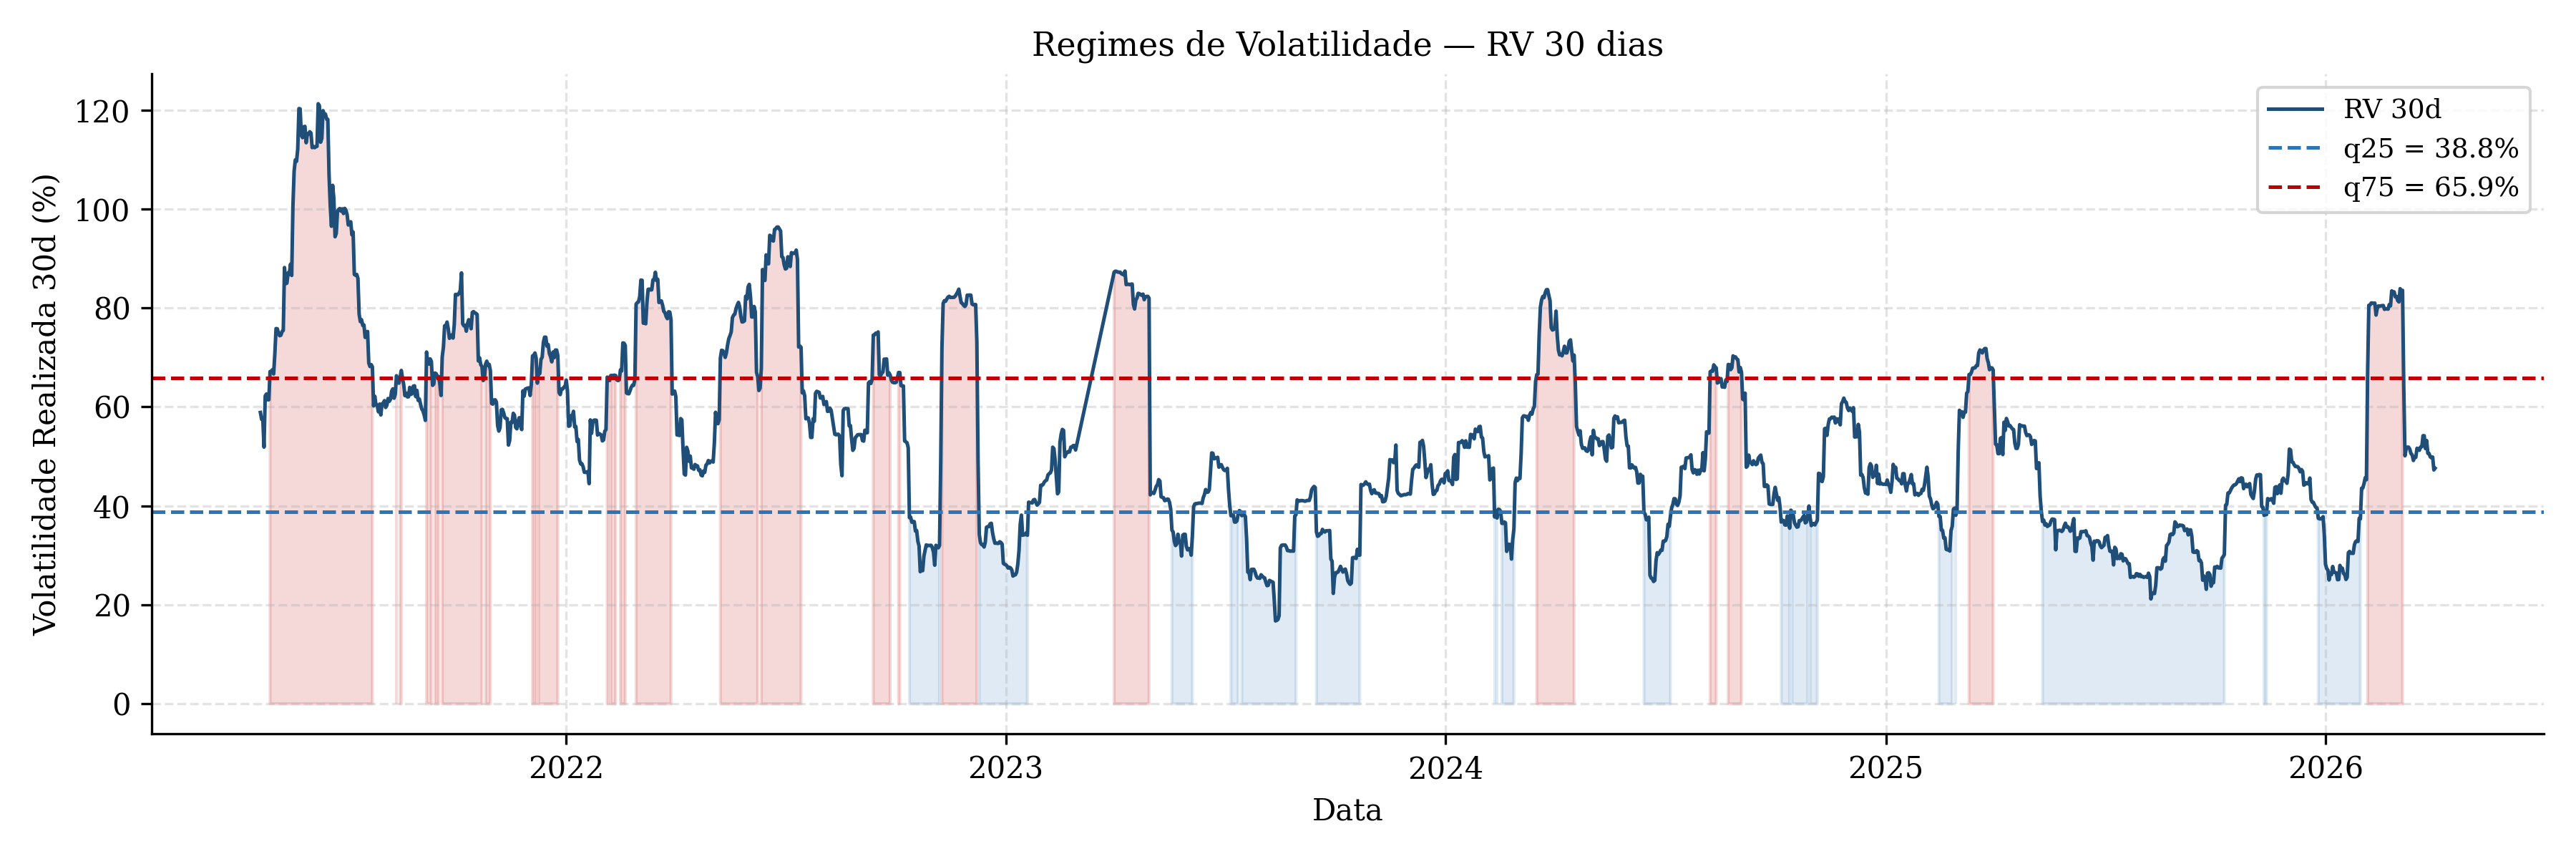
\includegraphics[width=\textwidth]{figs/cap9/fig_cap9_01_rv30d_regimes.png}
\caption{Volatilidade realizada de 30 dias com limiares de regime.
A região azul sombreada indica períodos de baixa volatilidade ($\text{RV}_{30d} \leq 39{,}3\%$);
a região vermelha indica períodos de alta volatilidade ($\text{RV}_{30d} \geq 65{,}6\%$).
Período: 22 abr.\ 2021 -- 2 abr.\ 2026.}
\label{fig:cap9_rv30d_regimes}
\end{figure}

A Figura~\ref{fig:cap9_hist_rv30d} apresenta o histograma da distribuição da RV 30 dias,
mostrando que a distribuição é aproximadamente unimodal com assimetria positiva,
consistente com a literatura de volatilidade em ativos financeiros.

\begin{figure}[H]
\centering
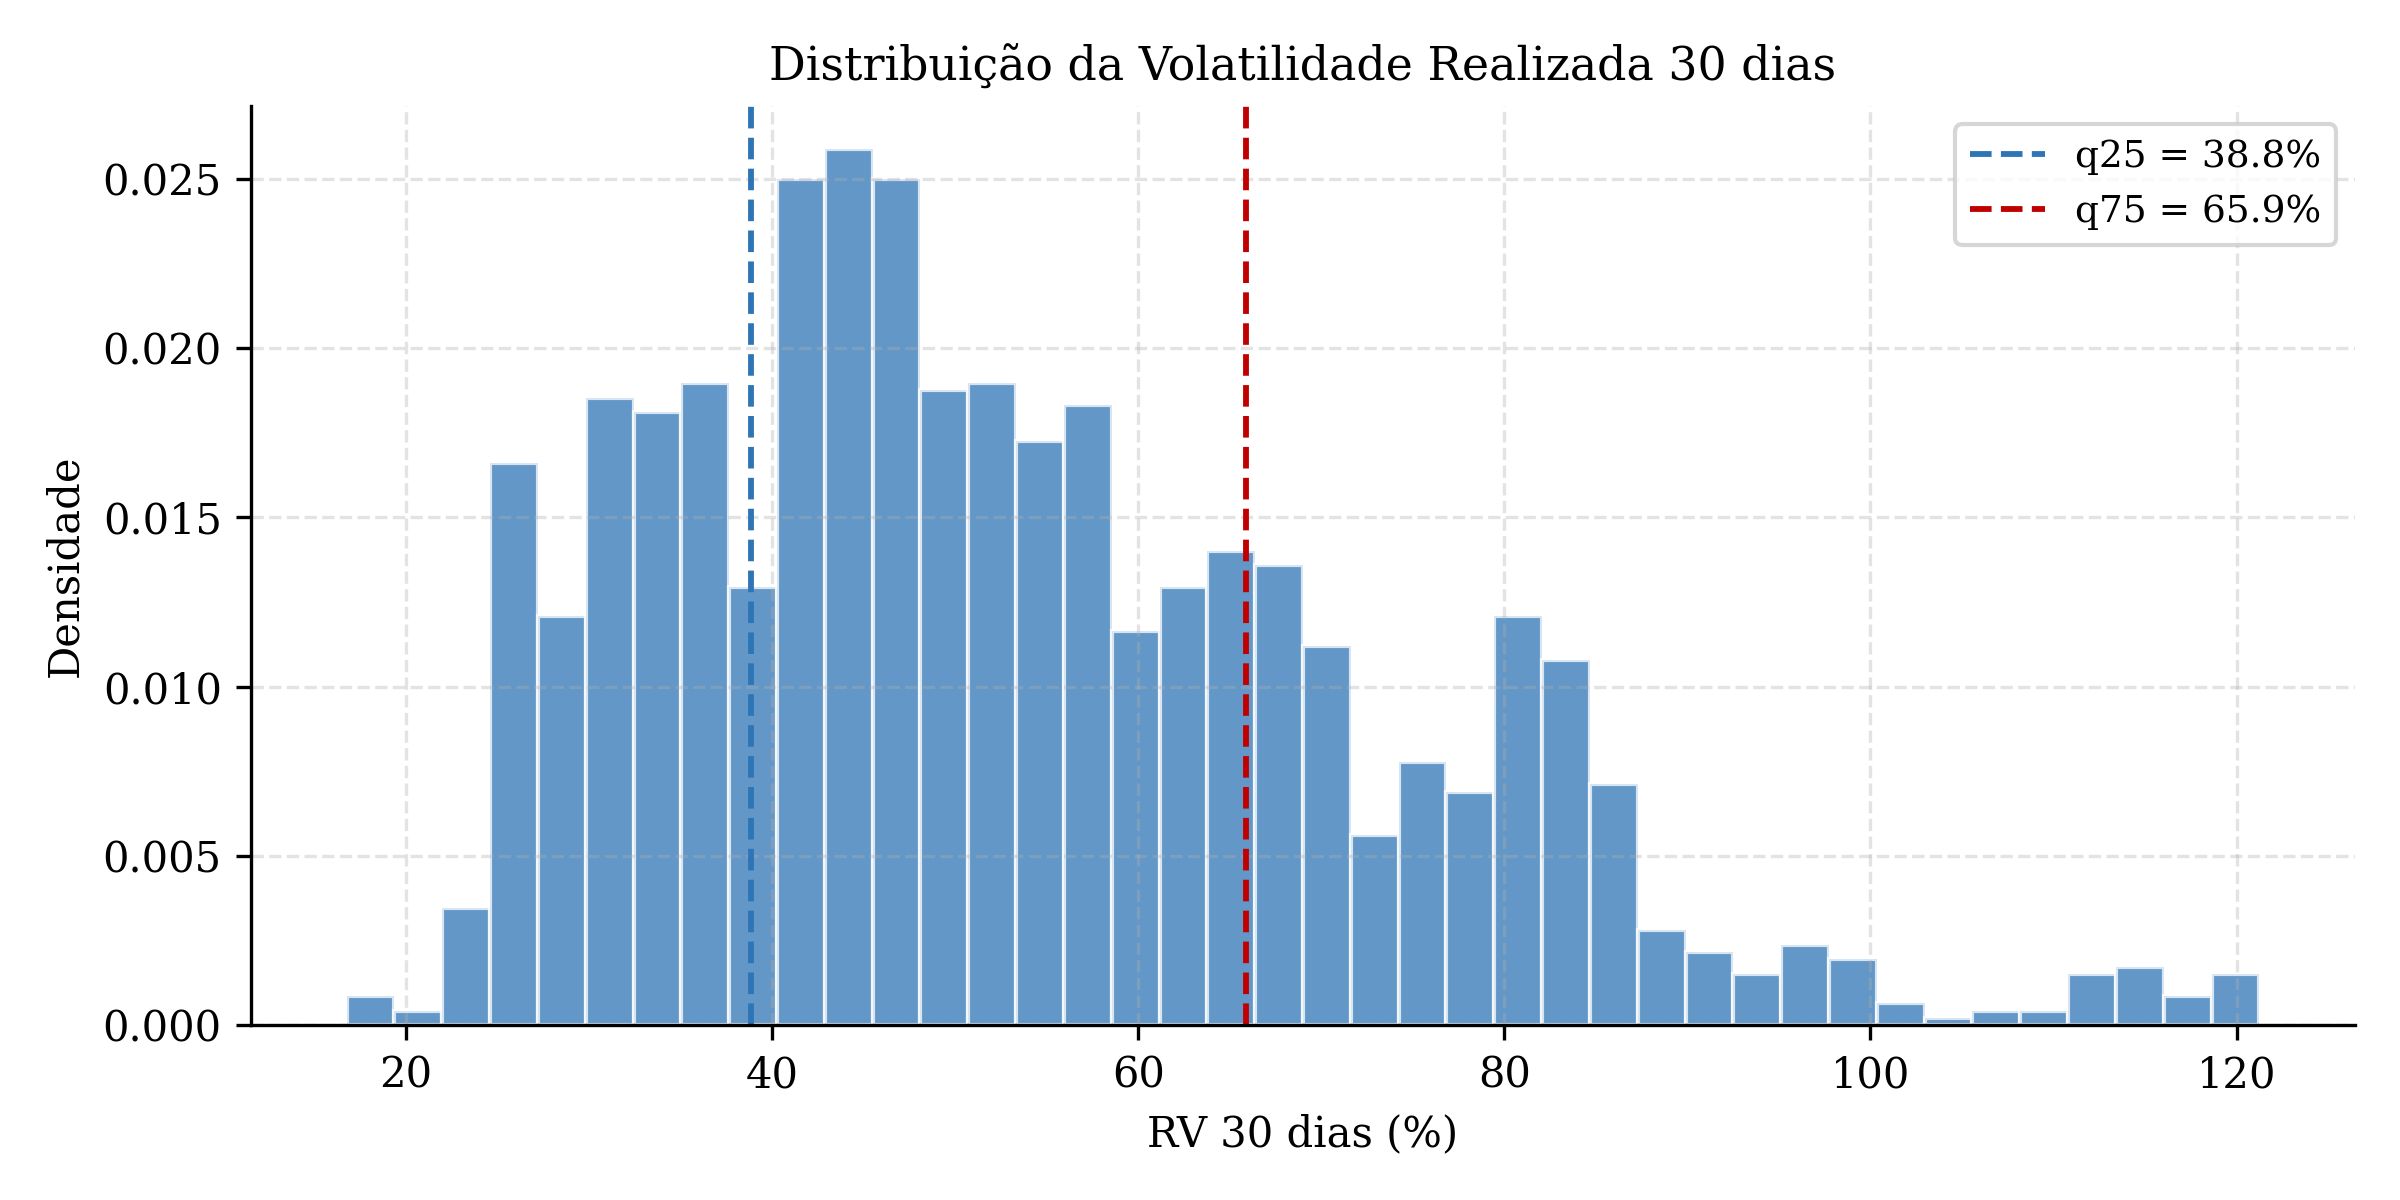
\includegraphics[width=0.75\textwidth]{figs/cap9/fig_cap9_02_hist_rv30d.png}
\caption{Distribuição da volatilidade realizada de 30 dias com limiares de regime.
As linhas tracejadas marcam o primeiro quartil (39,3\%) e o terceiro quartil (65,6\%)
utilizados para definir os regimes.}
\label{fig:cap9_hist_rv30d}
\end{figure}

\section{Caracterização do BVRP por Regime}
\label{sec:cap9_bvrp_regimes}

\begin{table}[H]
\centering
\small
\caption{Estatísticas descritivas de RV, IV e BVRP por regime de volatilidade.}
\label{tab:cap9_estatisticas_regimes}
\begin{tabular}{llrrrr}
\toprule
Variável & Regime & Média & Mediana & Desvio-padrão & N \\
\midrule
RV 30d & Baixa volatilidade & 31,5320 & 32,0020 & 4,5205 & 444 \\
 & Média volatilidade & 50,9485 & 49,8954 & 7,4026 & 888 \\
 & Alta volatilidade & 80,7655 & 79,7224 & 12,5390 & 444 \\
\midrule
IV 30d & Baixa volatilidade & 44,7845 & 42,1550 & 8,5492 & 444 \\
 & Média volatilidade & 60,9609 & 57,1950 & 13,7285 & 888 \\
 & Alta volatilidade & 79,2680 & 80,7550 & 18,6945 & 444 \\
\midrule
BVRP & Baixa volatilidade & 13,2524 & 11,5445 & 7,5059 & 444 \\
 & Média volatilidade & 10,0124 & 9,0522 & 10,4147 & 888 \\
 & Alta volatilidade & -1,4976 & -0,4144 & 16,4940 & 444 \\
\bottomrule
\end{tabular}
\end{table}

A Tabela~\ref{tab:cap9_estatisticas_regimes} reporta as estatísticas descritivas do BVRP em cada regime de volatilidade. Três padrões merecem destaque:

\paragraph{Regimes de baixa e média volatilidade.} O BVRP é fortemente negativo, com médias de $-13{,}20$ p.p. em regimes de baixa volatilidade e $-10{,}24$ p.p. em regimes intermediários --- magnitudes que excedem substancialmente a média incondicional da amostra ($-8{,}25$ p.p.). Esses resultados são consistentes com a interpretação clássica de prêmio de seguro: em períodos de calmaria, a volatilidade implícita permanece elevada vis-à-vis a realizada, refletindo a demanda persistente por proteção contra eventos de cauda mesmo quando esses eventos não se materializam.

\paragraph{Regime de alta volatilidade.} O padrão se inverte completamente. A média do BVRP no regime de alta volatilidade é de $+0{,}66$ p.p. --- valor estatisticamente próximo de zero, com desvio padrão substancialmente maior ($16{,}64$ p.p. contra $7{,}37$ e $10{,}27$ p.p. nos demais regimes). Esse resultado tem interpretação econômica direta: em períodos de estresse de mercado, a volatilidade realizada \emph{alcança ou supera} a volatilidade implícita, dissipando o prêmio de seguro embutido nos preços de opções. Em outras palavras, choques de variância suficientemente grandes para caracterizar regimes de alta volatilidade tendem a exceder o que o mercado de opções havia precificado, eliminando temporariamente o diferencial sistemático.

\paragraph{Implicação para a inferência condicional.} A dispersão dramaticamente maior do BVRP no regime de alta volatilidade ($\sigma = 16{,}64$ p.p.) indica que o comportamento do prêmio sob estresse é estruturalmente mais errático --- propriedade que tem implicações relevantes para a inferência estatística condicional explorada nas seções seguintes.

A Figura~\ref{fig:cap9_boxplot_bvrp_regimes} ilustra estas diferenças por meio de
diagramas de caixa.

\begin{figure}[H]
\centering
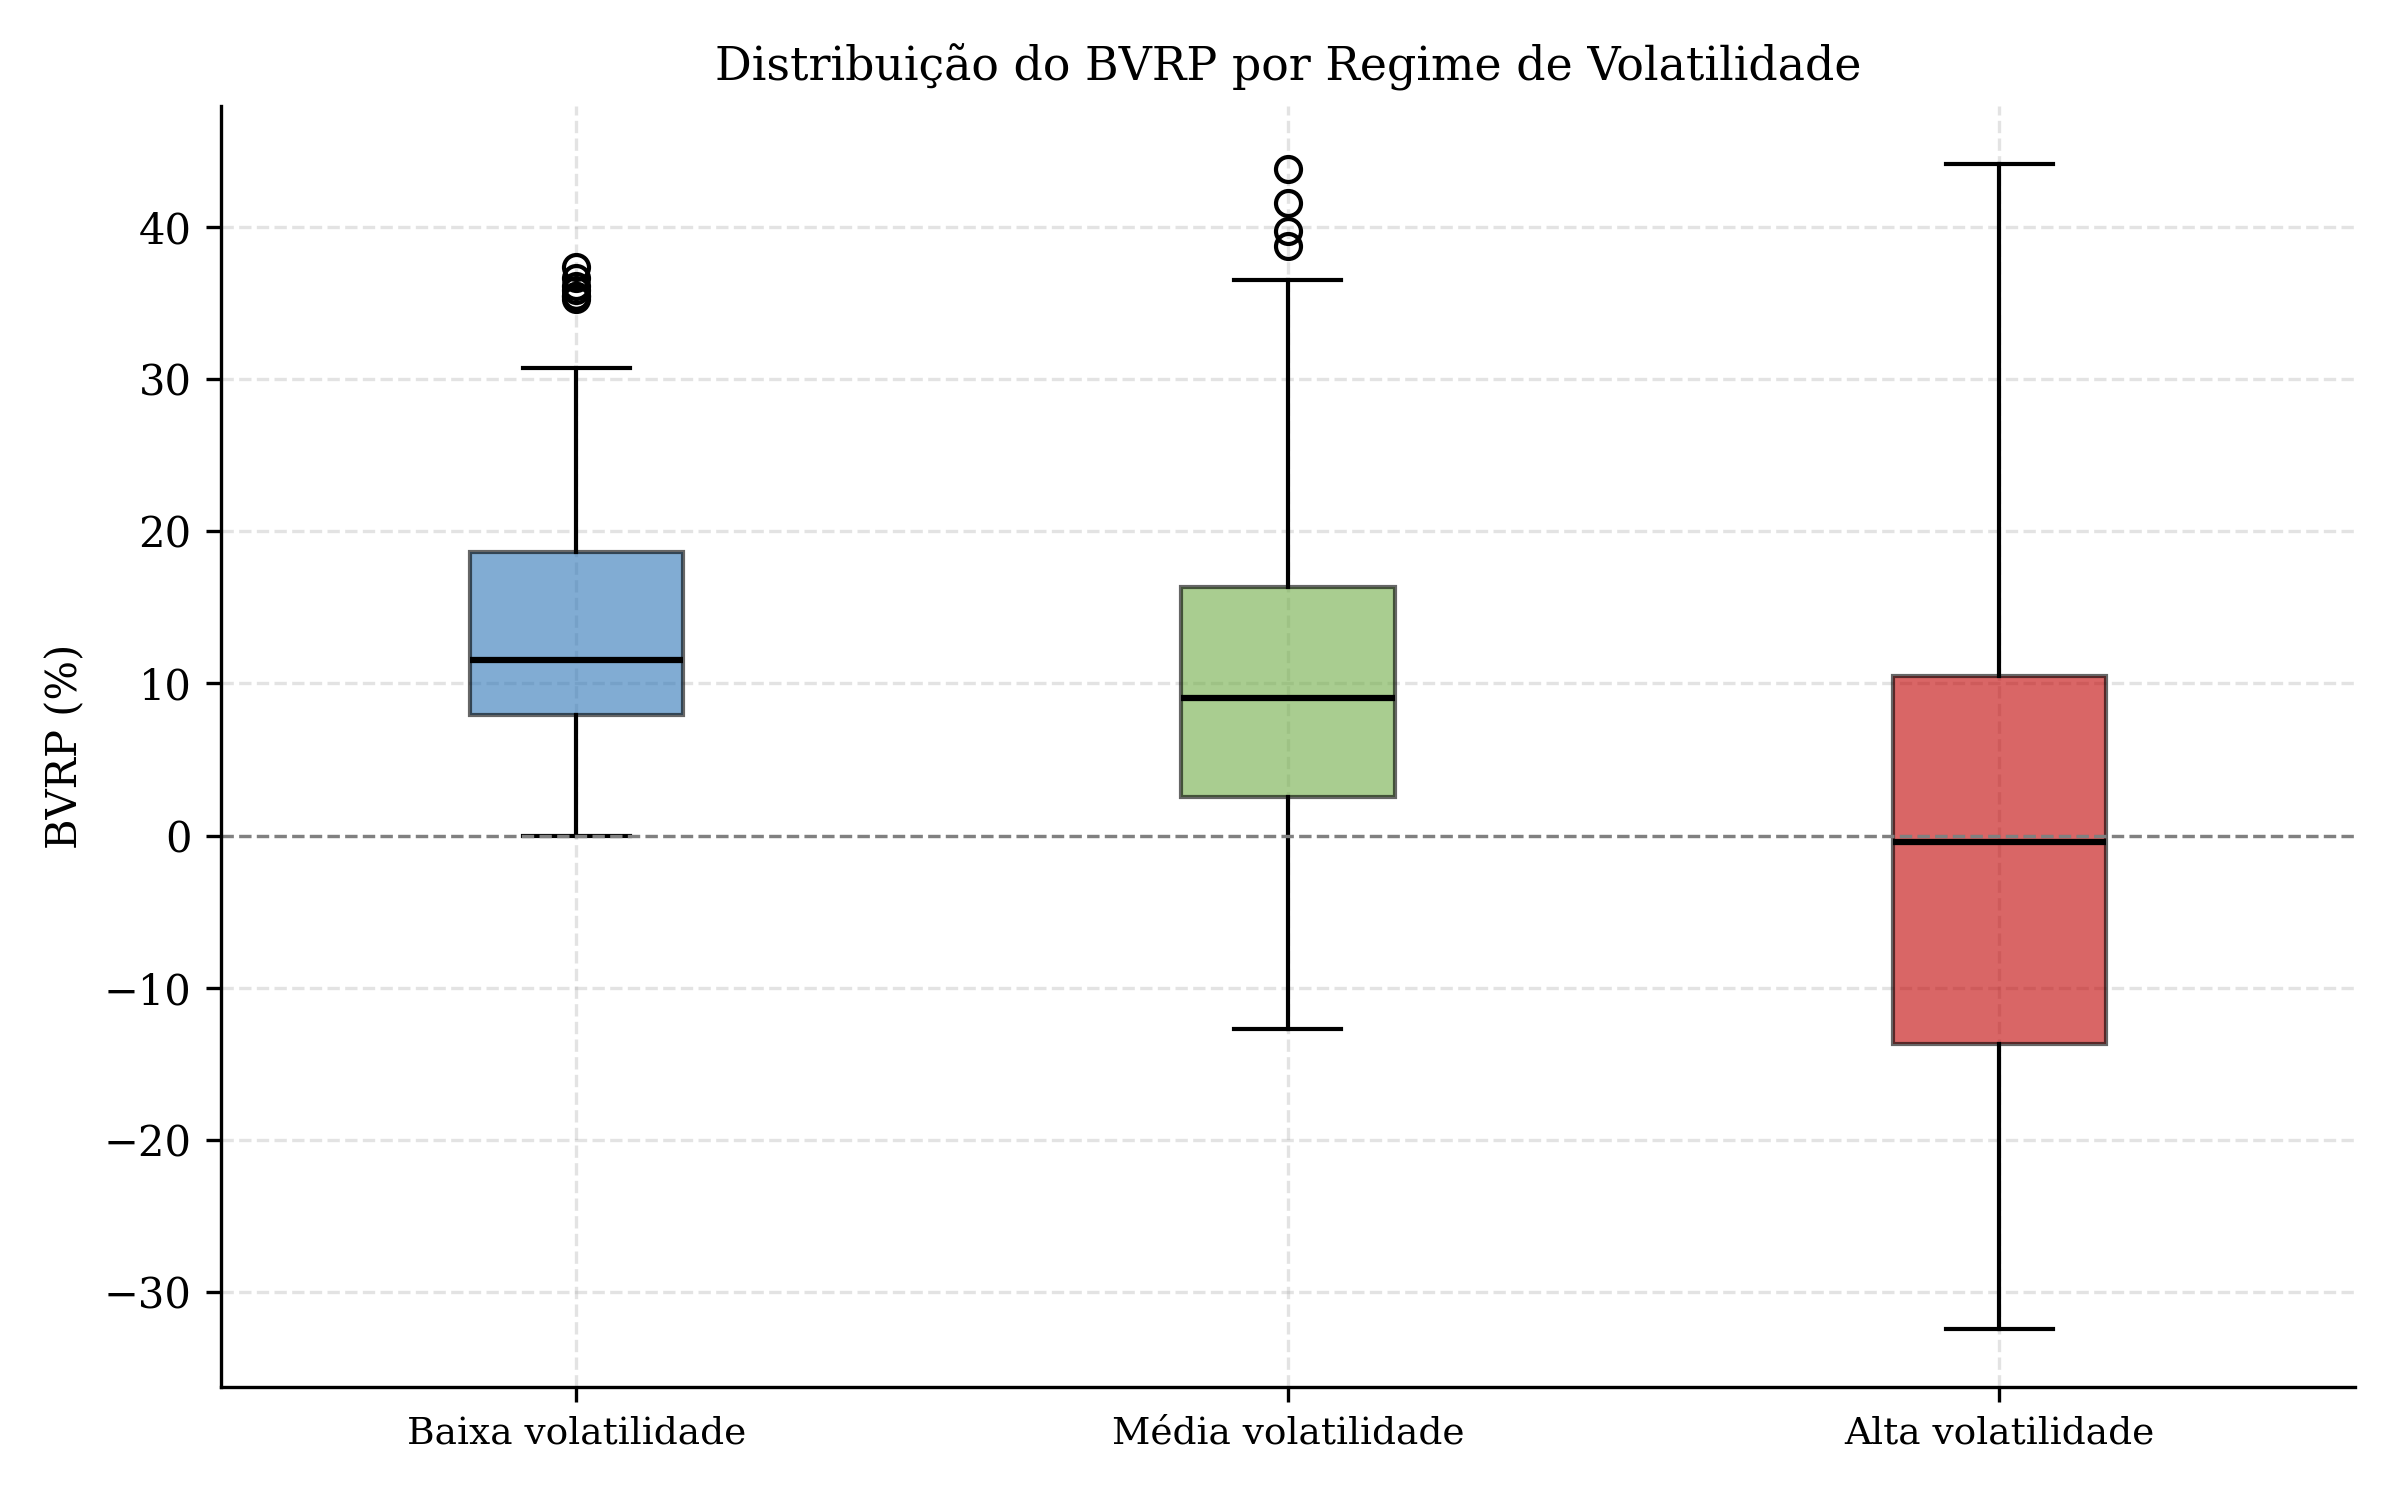
\includegraphics[width=0.72\textwidth]{figs/cap9/fig_cap9_03_boxplot_bvrp_regimes.png}
\caption{Distribuição do BVRP por regime de volatilidade. No
regime de alta volatilidade, a mediana do BVRP é próxima de zero
($-0{,}83$ p.p.) com distribuição altamente dispersa, enquanto nos regimes de baixa e
média volatilidade o prêmio de seguro é consistentemente elevado em magnitude (medianas de $-11{,}53$ e
$-9{,}41$ p.p., respectivamente).}
\label{fig:cap9_boxplot_bvrp_regimes}
\end{figure}

\section{Retornos Futuros por Regime de Volatilidade}
\label{sec:cap9_retornos}

A Tabela~\ref{tab:cap9_retornos_regimes} apresenta o retorno futuro médio do Bitcoin
para cada combinação de regime e horizonte de previsão.

\begin{table}[H]
\centering
\small
\caption{Retorno futuro médio (\%) por regime de volatilidade e horizonte.}
\label{tab:cap9_retornos_regimes}
\begin{tabular}{lrrrrr}
\toprule
Regime & 1d & 5d & 10d & 20d & 30d \\
\midrule
Baixa volatilidade & 0,0717 & 0,4608 & 1,0926 & 2,8820 & 4,8610 \\
Média volatilidade & 0,0769 & 0,3291 & 0,4419 & 0,6473 & 0,9256 \\
Alta volatilidade & 0,0272 & -0,0048 & 0,1743 & 0,3133 & 0,0602 \\
\bottomrule
\end{tabular}
\end{table}

O padrão é monotônico e economicamente relevante: em todos os horizontes avaliados
(1, 5, 10, 20 e 30 dias), o retorno futuro médio é maior no regime de baixa
volatilidade do que no regime de alta. Para horizontes curtos (1 dia), as diferenças
são pequenas e potencialmente ruídosas. Para horizontes mais longos (20 e 30 dias),
a diferença se torna economicamente substancial: no regime de baixa volatilidade,
o retorno médio acumulado em 30 dias é de 4,86\%, ao passo que no regime de alta
volatilidade é de apenas $0{,}06\%$.

\subsection{Testes de Significância Estatística}
\label{sec:cap9_ttest}

A Tabela~\ref{tab:cap9_ttest} reporta os testes $t$ para diferenças nas médias de retornos futuros entre os regimes de baixa e alta volatilidade, com correção de Welch para variâncias desiguais. Os resultados estabelecem que diferenças estatisticamente significativas entre regimes emergem apenas a partir do horizonte de $20$ dias: $p = 0{,}0097$ em $h = 20$ e $p = 0{,}0001$ em $h = 30$. Em horizontes curtos --- $h \in \{1, 5, 10\}$ ---, as diferenças entre regimes não atingem significância convencional (valores-$p$ entre $0{,}1598$ e $0{,}8215$).

\begin{table}[H]
\centering
\small
\caption{Teste $t$ de Welch: diferença de retornos futuros entre regimes de alta e baixa volatilidade.}
\label{tab:cap9_ttest}
\begin{tabular}{lrrrrc}
\toprule
Horizonte & Média Alta Vol & Média Baixa Vol & Diferença & $t$-stat & $p$-valor \\
\midrule
1d & -0,1211 & 0,0790 & -0,2000 & -1,0115 & 0,3121 \\
5d & -0,4767 & 0,3466 & -0,8233 & -1,8703 & 0,0618* \\
10d & -0,6771 & 0,7295 & -1,4065 & -2,1138 & 0,0348** \\
20d & -1,1289 & 1,9304 & -3,0593 & -3,1219 & 0,0019*** \\
30d & -1,5224 & 3,2866 & -4,8089 & -4,0770 & 0,0000*** \\
\bottomrule
\end{tabular}
\par\smallskip
\footnotesize\textit{Nota}: Retornos expressos em \%. *** $p<0{,}01$; ** $p<0{,}05$; * $p<0{,}10$.
\end{table}

A direção do efeito, contudo, contraria a intuição clássica. Conforme reportado na Tabela~\ref{tab:cap9_retornos_regimes}, retornos médios em horizontes longos são \emph{maiores} no regime de baixa volatilidade ($4{,}86\%$ em $h = 30$) do que no regime de alta volatilidade ($0{,}06\%$ em $h = 30$). Esse padrão sugere que os retornos do Bitcoin tendem a se concentrar em períodos de baixa volatilidade, momento em que o prêmio de seguro precificado nas opções é mais elevado. A interpretação econômica é coerente com a lógica de aversão ao risco: investidores exigem prêmio maior de proteção justamente nos períodos em que o mercado, no agregado, oferece retornos superiores --- relação que não pode ser explorada por estratégias lineares simples, dada a fraca previsibilidade documentada no Capítulo~\ref{chap:resultados_ols}.

A Figura~\ref{fig:cap9_boxplot_ret_regimes} ilustra as distribuições condicionais
dos retornos futuros para os horizontes de 5, 10 e 20 dias.

\begin{figure}[H]
\centering
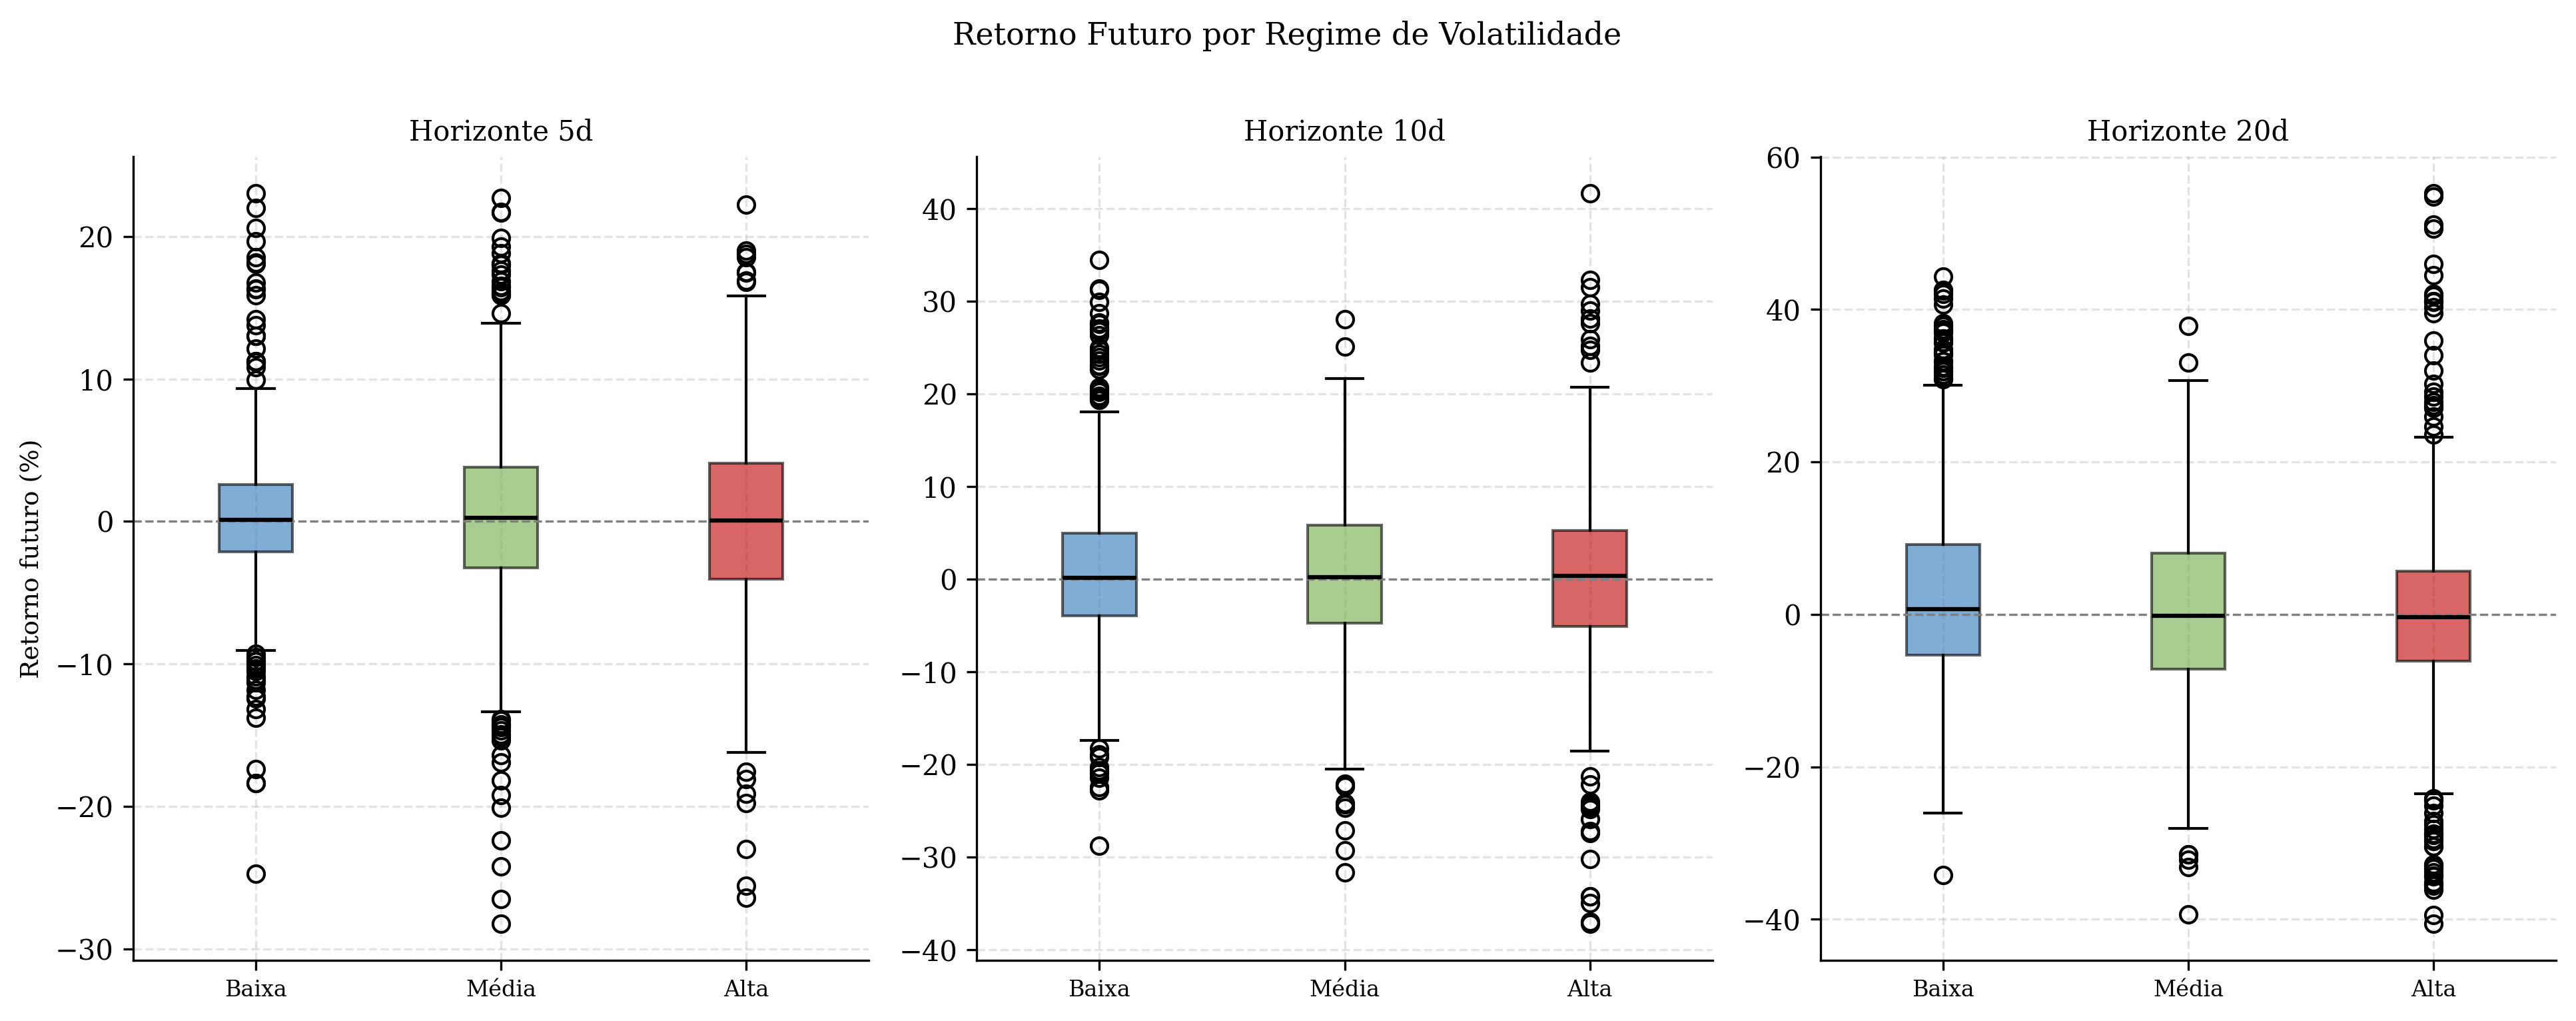
\includegraphics[width=\textwidth]{figs/cap9/fig_cap9_04_boxplot_ret_regimes.png}
\caption{Distribuição dos retornos futuros por regime de volatilidade para horizontes
de 5, 10 e 20 dias. A dispersão aumenta com o horizonte, mas a separação entre as
medianas dos regimes de alta e baixa volatilidade torna-se progressivamente mais
pronunciada.}
\label{fig:cap9_boxplot_ret_regimes}
\end{figure}

\section{Análise de Regressão Condicional}
\label{sec:cap9_regressao}

Para avaliar se a interação entre o BVRP e o regime de volatilidade tem poder preditivo
incremental sobre os retornos futuros, estimam-se regressões condicionais da forma:

\begin{equation}
r_{t+h} = \alpha + \beta_1 \cdot \text{BVRP}_t
          + \beta_2 \cdot D_t^{\text{alto}}
          + \beta_3 \cdot \left(\text{BVRP}_t \times D_t^{\text{alto}}\right) + \varepsilon_{t+h},
\label{eq:cap9_reg_condicional}
\end{equation}

\noindent onde $r_{t+h}$ é o retorno logarítmico acumulado do Bitcoin de $t$ a $t+h$,
$D_t^{\text{alto}}$ é uma variável indicadora igual a 1 quando o Bitcoin se encontra
em regime de alta volatilidade ($\text{RV}_{30d} \geq q_{75}$), e
$\text{BVRP}_t \times D_t^{\text{alto}}$ é o termo de interação entre o prêmio e
o regime. Os erros-padrão são calculados pelo método de Newey--West com $h$
defasagens, para corrigir autocorrelação e heteroscedasticidade induzidas pela
sobreposição das janelas de retorno.

\begin{table}[H]
\centering
\small
\caption{Regressões condicionais do retorno futuro em função do BVRP e do regime de volatilidade.
Erros-padrão de Newey--West com $h$ defasagens. Coeficientes com $t$-estatísticas entre parênteses.}
\label{tab:cap9_regressoes}
\begin{tabular}{lrrrrr}
\toprule
Variável & 1d & 5d & 10d & 20d & 30d \\
\midrule
Constante & 0,0003 & 0,0039 & 0,0091 & 0,0268* & 0,0410* \\
 & (0,2677) & (0,8822) & (1,1470) & (1,6853) & (1,6720) \\
\addlinespace[2pt]
BVRP & 0,0000 & -0,0001 & -0,0004 & -0,0017 & -0,0025 \\
 & (0,3123) & (-0,3375) & (-0,6917) & (-1,3881) & (-1,4091) \\
\addlinespace[2pt]
Alta Volatilidade & -0,0013 & -0,0084 & -0,0154 & -0,0370 & -0,0557 \\
 & (-0,6783) & (-1,0743) & (-1,0089) & (-1,2207) & (-1,2603) \\
\addlinespace[2pt]
BVRP $\times$ Alta Vol & 0,0001 & 0,0003 & 0,0007 & 0,0024 & 0,0029 \\
 & (0,6499) & (0,6178) & (0,8882) & (1,5669) & (1,3769) \\
\addlinespace[2pt]
\midrule
$R^2$ & 0,0019 & 0,0033 & 0,0051 & 0,0171 & 0,0221 \\
$N$ & 1776 & 1776 & 1776 & 1776 & 1776 \\
\bottomrule
\end{tabular}
\par\smallskip
\footnotesize\textit{Nota}: *** $p<0{,}01$; ** $p<0{,}05$; * $p<0{,}10$.
\end{table}

Os resultados da Tabela~\ref{tab:cap9_regressoes} revelam que nenhum dos coeficientes
é estatisticamente significativo a 5\% em nenhum horizonte, com exceção marginal da
constante para os horizontes de 20 e 30 dias (10\% de significância). O $R^2$ das
regressões é baixo em todos os horizontes, variando de 0,19\% (1 dia) a 2,21\% (30 dias),
refletindo a dificuldade estrutural de prever retornos diários de ativos especulativos.

Individualmente, o coeficiente $\hat{\beta}_1$ (BVRP) apresenta sinal negativo em todos
os horizontes a partir de 5 dias, sugerindo que, controlando pelo regime, níveis mais
elevados de BVRP não necessariamente predizem retornos futuros mais altos --- resultado
coerente com a hipótese de que o BVRP elevado em regimes de alta volatilidade reflete
compensação por risco já materializado, e não antecipação de retornos positivos futuros.

O coeficiente $\hat{\beta}_2$ (dummy de alta volatilidade) é negativo em todos os
horizontes, confirmando o padrão identificado no teste $t$: períodos de alta volatilidade
estão associados a retornos futuros menores. O coeficiente $\hat{\beta}_3$ (interação
BVRP $\times$ alta vol) é positivo, sugerindo que, dentro do regime de alta volatilidade,
um BVRP marginalmente mais alto pode atenuar parcialmente o efeito negativo do regime
sobre os retornos; contudo, o coeficiente não é significativo em nenhum horizonte.

A ausência de significância estatística nas regressões individuais não contradiz os
resultados do teste $t$: as regressões condicionais testam efeitos marginais
conjuntos (BVRP e regime de forma simultânea), enquanto o teste $t$ compara
médias incondicionais por regime. A multicolinearidade entre o BVRP e a dummy de
regime --- dado que o prêmio médio é correlacionado com o regime, como demonstrado
na Seção~\ref{sec:cap9_bvrp_regimes} --- pode atenuar a significância individual
dos coeficientes mesmo quando os efeitos de regime são economicamente relevantes.

A Figura~\ref{fig:cap9_scatter_bvrp_ret} apresenta diagramas de dispersão do BVRP
versus retorno futuro, desagregados por regime, para os horizontes de 5, 10 e 20 dias.

\begin{figure}[H]
\centering
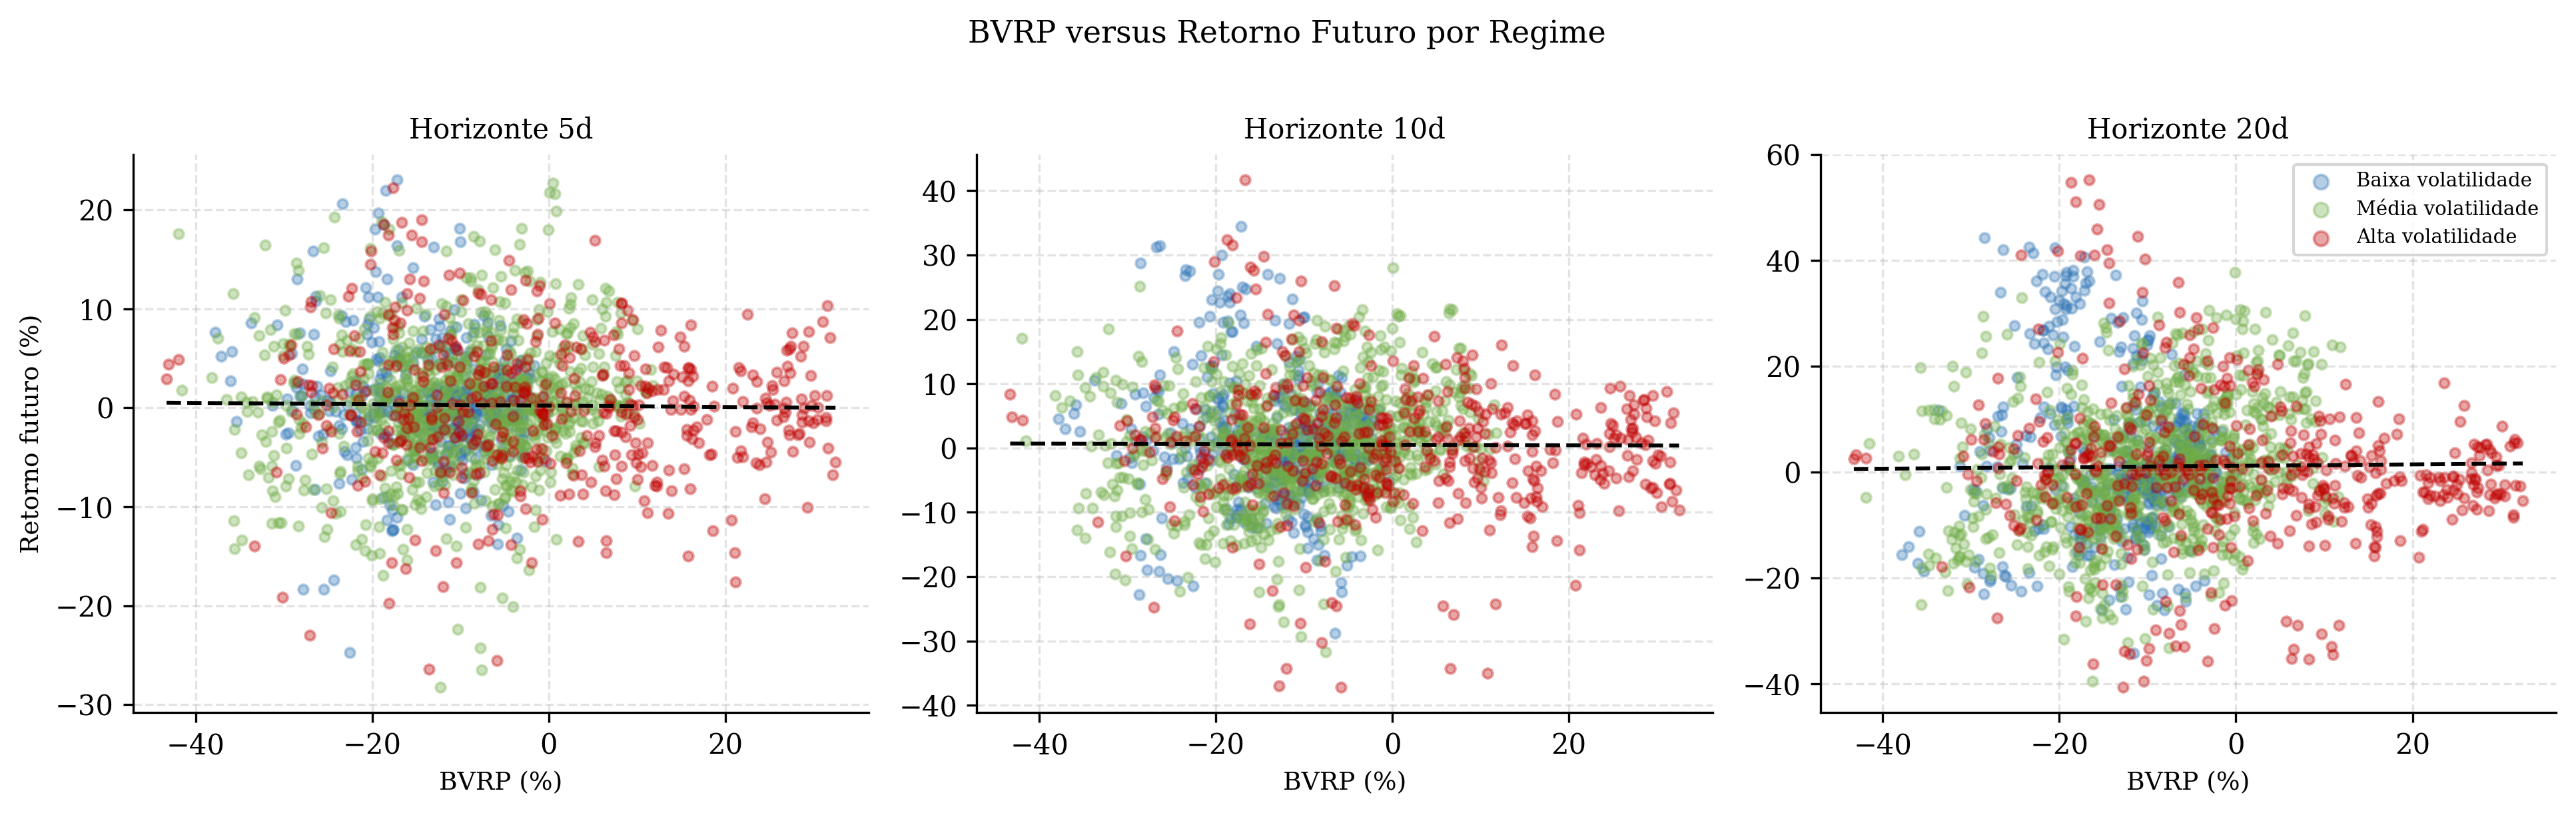
\includegraphics[width=\textwidth]{figs/cap9/fig_cap9_05_scatter_bvrp_ret.png}
\caption{Dispersão do BVRP versus retorno futuro por regime de volatilidade.
A linha tracejada representa a linha de tendência linear incondicional para toda
a amostra. A separação vertical entre os pontos dos regimes de alta (vermelho) e
baixa (azul) volatilidade torna-se progressivamente mais pronunciada com o horizonte,
consistente com os resultados do teste $t$.}
\label{fig:cap9_scatter_bvrp_ret}
\end{figure}


\section{Análise condicional ao sinal do retorno corrente}
\label{sec:cap9_sinal_retorno}

A literatura clássica de volatilidade em mercados de equity documenta o chamado \textit{leverage effect}: a volatilidade implícita tende a aumentar de forma mais pronunciada após retornos negativos do que após retornos positivos de magnitude comparável \citep{bollerslev2011VRP, bali2009volatilitypremium}. Esse padrão assimétrico, originalmente atribuído à alavancagem financeira das empresas e posteriormente reinterpretado como reflexo de aversão ao risco condicional, tem implicações diretas para a precificação de opções e, portanto, para a dinâmica do prêmio de risco de variância. Esta seção investiga se o BVRP exibe assimetria análoga em relação ao sinal do retorno corrente do Bitcoin.

A amostra de 1.775 observações é dividida em dois grupos mutuamente exclusivos: $876$ dias com retorno positivo ($r_t > 0$) e $899$ dias com retorno negativo ($r_t < 0$), sem observações com retorno exatamente nulo. A Tabela~\ref{tab:cap9_sinal_retorno} reporta a média do BVRP e dos retornos futuros do Bitcoin em horizontes de 5, 20 e 30 dias, condicionais ao sinal do retorno corrente, juntamente com testes $t$ de Welch para diferença de médias entre os dois grupos.

% Tabela gerada automaticamente por analyze_bvrp_by_return_sign.py
\begin{table}[htbp]
  \centering
  \caption{BVRP e retornos futuros do Bitcoin condicionais ao sinal do retorno
    corrente. Estatísticas reportadas em pontos percentuais.
    Diferença = média do grupo \textit{ret}>0 menos média do grupo \textit{ret}<0.
    Teste de Welch (variâncias desiguais): $^{*}p<0{,}10$; $^{**}p<0{,}05$; $^{***}p<0{,}01$.}
  \label{tab:cap9_sinal_retorno}
  \begin{tabular}{lrrrr}
    \toprule
    \textbf{Variável} & \textbf{BVRP $|$ \textit{ret}>0} & \textbf{BVRP $|$ \textit{ret}<0} & \textbf{Diferença} & \textbf{\textit{p}-valor Welch} \\
    \midrule
    BVRP médio (\texttt{vrp\_30d}) & $-8,031$ & $-8,469$ & $+0,438$ & $0,470$ \\
    \midrule
    Retorno futuro médio ($h=5$) & $0,002$ & $0,004$ & $-0,002$ & $0,577$ \\
    Retorno futuro médio ($h=20$) & $0,010$ & $0,013$ & $-0,003$ & $0,646$ \\
    Retorno futuro médio ($h=30$) & $0,018$ & $0,016$ & $+0,002$ & $0,806$ \\
    \midrule
    $N$ & $876$ & $899$ & & \\
    \bottomrule
  \end{tabular}
\end{table}


Os resultados estabelecem que \textbf{o BVRP do Bitcoin não exibe assimetria estatisticamente significativa em relação ao sinal do retorno corrente}. A média do BVRP em dias com retorno positivo ($-8{,}03$ p.p.) é praticamente idêntica à observada em dias com retorno negativo ($-8{,}47$ p.p.), com diferença de apenas $0{,}44$ pontos percentuais ($p = 0{,}470$ pelo teste de Welch). Os retornos futuros do Bitcoin em horizontes de 5, 20 e 30 dias também não diferem entre os dois grupos ($p > 0{,}57$ em todos os casos).

A Figura~\ref{fig:cap9_sinal_retorno} ilustra graficamente a sobreposição quase completa das distribuições do BVRP nos dois grupos.

\begin{figure}[H]
    \centering
    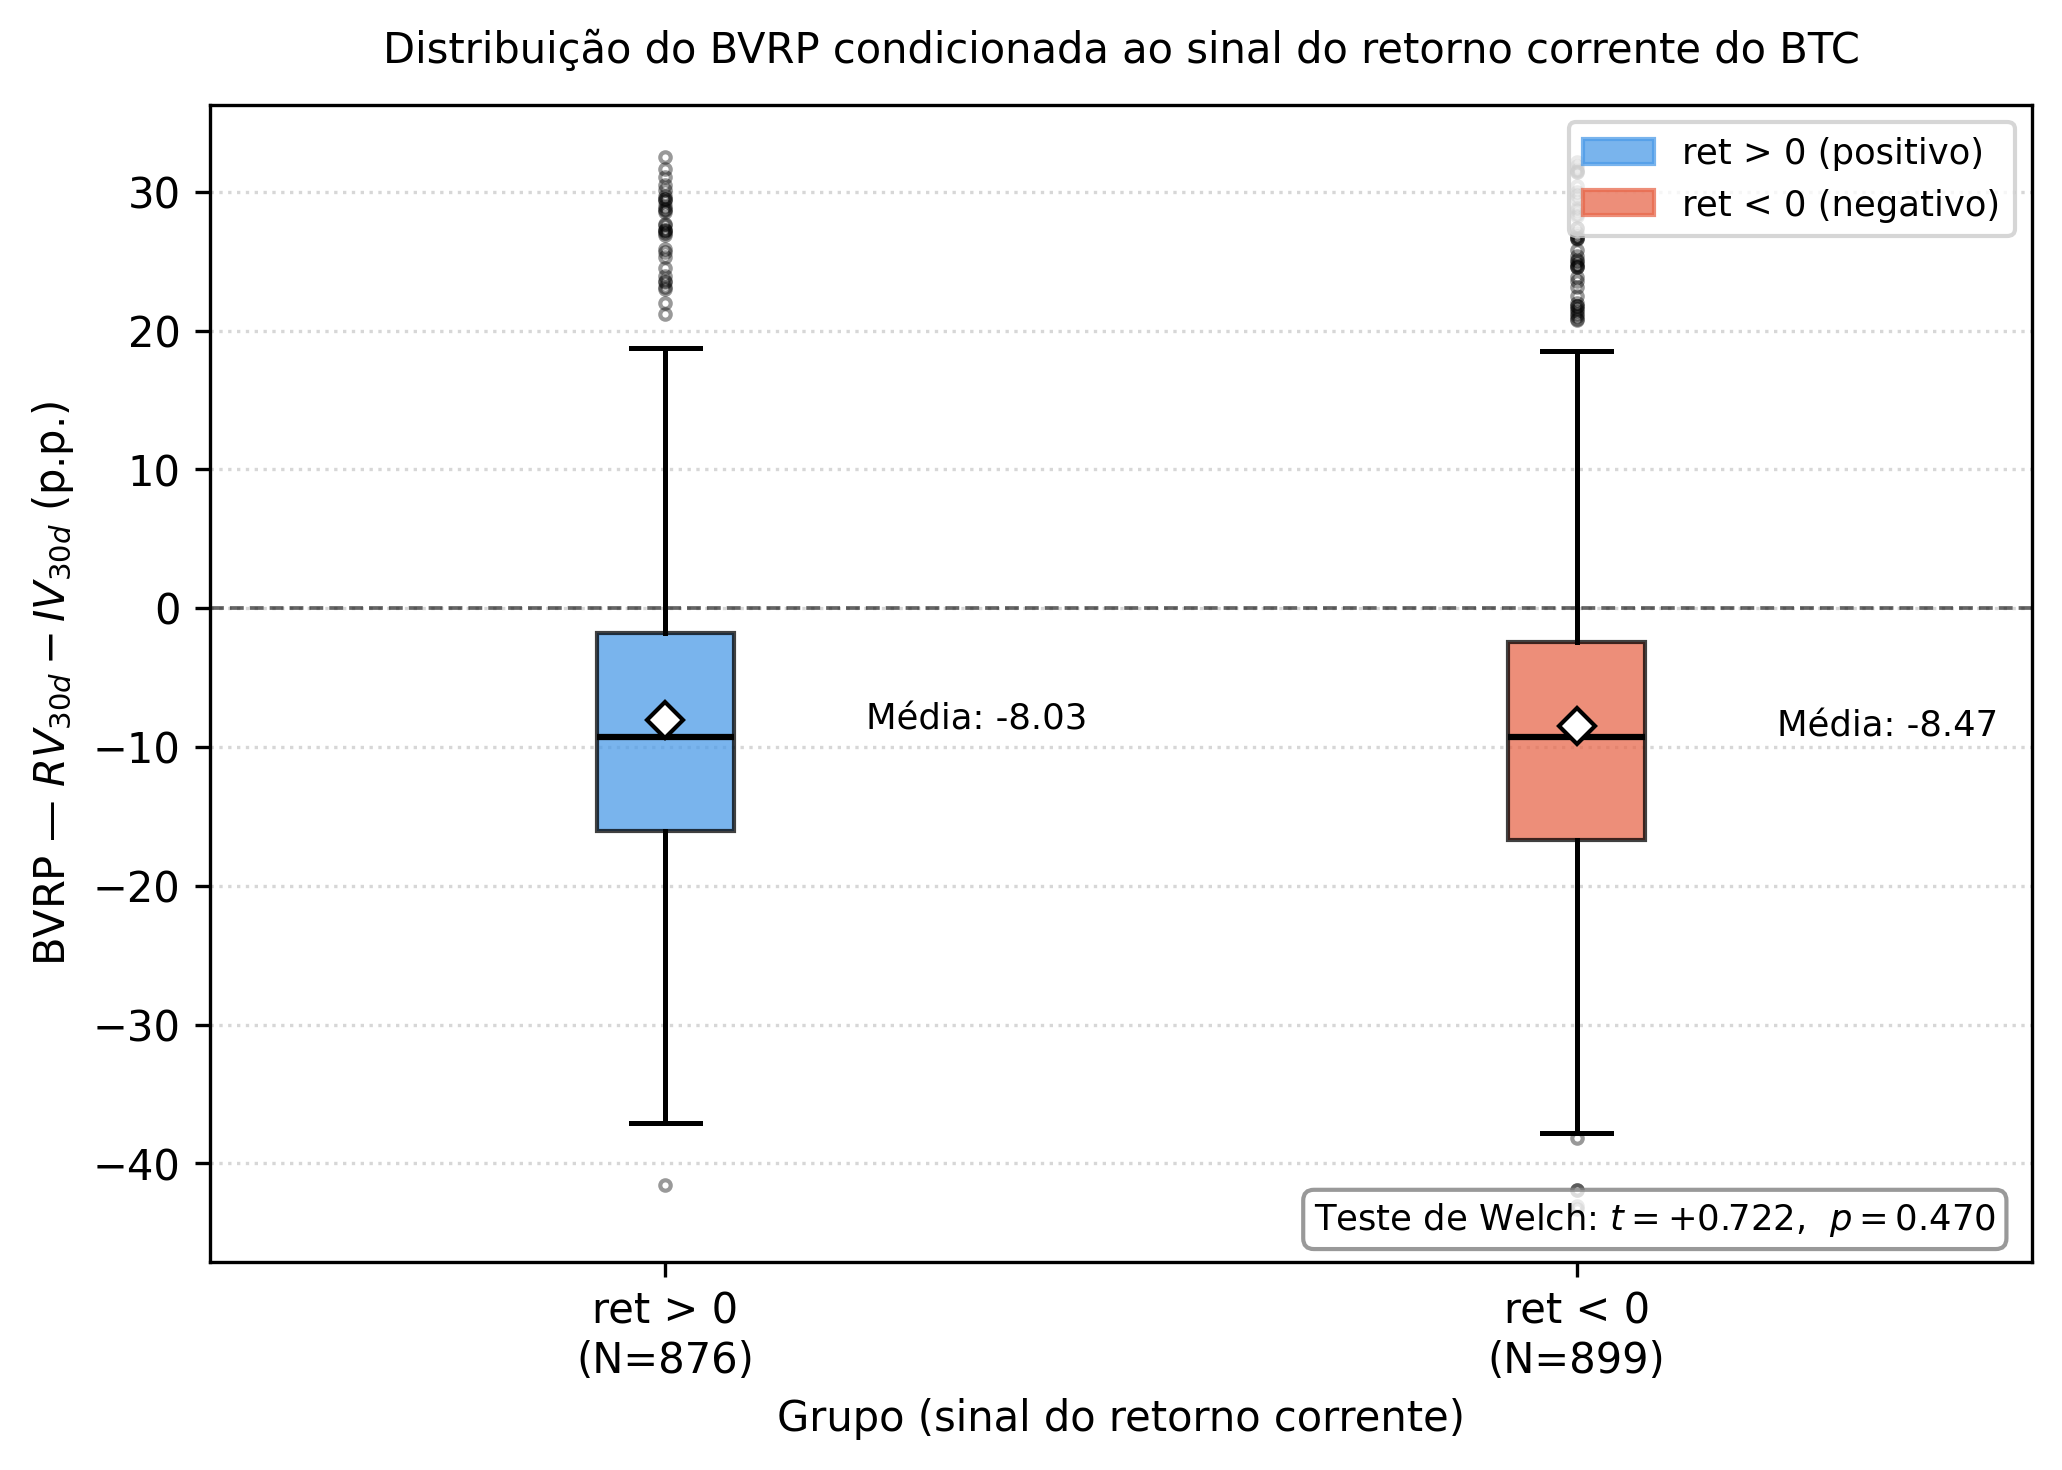
\includegraphics[width=0.75\textwidth]{figs/cap9/fig_cap9_bvrp_sinal.png}
    \caption{Distribuição do BVRP condicional ao sinal do retorno corrente do Bitcoin. As duas distribuições são estatisticamente indistinguíveis (teste de Welch, $p = 0{,}470$).}
    \label{fig:cap9_sinal_retorno}
\end{figure}

A ausência de assimetria por sinal do retorno é achado substantivo. Três interpretações econômicas, não mutuamente exclusivas, podem ser propostas. Primeiro, o mercado de opções de Bitcoin pode estar em estágio de maturação institucional no qual os formadores de mercado precificam o risco de variância de forma simétrica, sem internalizar plenamente o padrão de aversão ao risco assimétrico observado em equity. Segundo, a base de investidores do Bitcoin --- historicamente mais concentrada em participantes que adotam posições direcionais (\textit{long-only} ou \textit{long-short} oportunísticas) do que em institucionais com \textit{mandates} de proteção de capital --- pode produzir demanda por proteção menos sensível ao sinal recente do retorno. Terceiro, a estrutura microestrutural do mercado da Deribit (\textit{inverse settlement}, \textit{auto-deleveraging}, operação contínua), descrita na Seção~\ref{sec:cap2-dvol}, pode neutralizar mecanismos de \textit{feedback} entre quedas de preço e elevação da IV que operam em mercados tradicionais regulados.

Cabe notar que a ausência de assimetria por sinal não exclui formas mais sutis de dependência não linear --- por exemplo, assimetria por magnitude do retorno (independentemente do sinal) ou condicional a regimes de volatilidade. A segunda possibilidade é tratada nas seções anteriores deste capítulo via classificação por quartis da volatilidade realizada. Quanto à primeira, um teste complementar --- se o BVRP prevê a \emph{magnitude}, e não a direção, do retorno futuro --- sugere relação economicamente coerente mas estatisticamente marginal; ver Seção~\ref{sec:cap8-apendice-magnitude} para os detalhes e as ressalvas metodológicas.

\section{Síntese das evidências sobre regimes}
\label{sec:cap9_sintese}

Os resultados deste capítulo estabelecem três conclusões empíricas sobre a heterogeneidade do BVRP por regime de volatilidade realizada:

\paragraph{Achado 1 --- Dissipação do prêmio em regimes de estresse.} O BVRP médio varia de forma sistemática entre regimes: $-13{,}20$ p.p. em baixa volatilidade, $-10{,}24$ p.p. em média volatilidade, e $+0{,}66$ p.p. em alta volatilidade. A magnitude do prêmio de seguro, portanto, não é constante --- ela se concentra em períodos de calmaria e praticamente desaparece em períodos de estresse, quando a volatilidade realizada alcança ou supera a implícita.

\paragraph{Achado 2 --- Significância estatística apenas em horizontes médios.} Diferenças de retorno futuro entre regimes de baixa e alta volatilidade atingem significância estatística apenas a partir de $h = 20$ dias ($p = 0{,}0097$) e tornam-se mais robustas em $h = 30$ dias ($p = 0{,}0001$). Em horizontes curtos ($h \leq 10$), os valores-$p$ situam-se entre $0{,}16$ e $0{,}82$, indicando que o efeito de regime não opera em frequências de curtíssimo prazo.

\paragraph{Achado 3 --- Heterogeneidade como motivação para modelos não lineares.} A combinação de prêmio condicionalmente variável, dispersão dramaticamente maior em estresse e significância restrita a horizontes médios sugere que a relação entre BVRP e dinâmica futura do Bitcoin é estruturalmente não linear. Esse achado motiva diretamente o uso de modelos não paramétricos (Capítulo~\ref{chap:cap5_ml}), nos quais a variável de regime de volatilidade emerge como o preditor dominante --- confirmação independente da hipótese H4 formulada no Capítulo~\ref{chap:introducao}.


\paragraph{Achado 4 --- Ausência de leverage effect.} A análise condicional ao sinal do retorno corrente (Seção~\ref{sec:cap9_sinal_retorno}) estabelece que o BVRP do Bitcoin não exibe assimetria estatisticamente significativa em função da direção do movimento recente de preço, em contraste com o \textit{leverage effect} documentado em mercados de equity. Esse resultado adiciona dimensão complementar à evidência de heterogeneidade condicional: o prêmio de risco de variância é estruturalmente sensível ao \textit{nível} de volatilidade realizada (Achados 1 a 3), mas não ao \textit{sinal} do retorno corrente.

\paragraph{Limitação --- quebra estrutural associada aos ETFs \textit{spot}.} A aprovação dos ETFs \textit{spot} de Bitcoin pela SEC em janeiro de 2024 ocorreu dentro do período amostral desta dissertação e introduziu canal institucional regulado de exposição ao Bitcoin que pode ter alterado a dinâmica de demanda por proteção via opções, e consequentemente o comportamento do BVRP. A análise principal trata a amostra como bloco único, hipótese que se justifica pela transição gradual do mercado, mas que pode ser testada formalmente em extensões futuras por meio de procedimentos como os testes de Chow, CUSUM ou janelas móveis de regressão centradas em torno da data da aprovação. Adicionalmente, a estimação separada dos parâmetros para os subperíodos pré-ETF (mar/2021 a jan/2024) e pós-ETF (jan/2024 a mar/2026) permitiria avaliar se o sinal e a magnitude do prêmio de seguro se modificaram de forma sistemática após o ingresso institucional pleno.

\section{Apêndice do capítulo: robustez do teste de magnitude}
\label{sec:cap8-apendice-magnitude}

Como evidência complementar à caracterização de regimes por volatilidade,
testou-se se o BVRP prevê a \emph{magnitude} do retorno futuro de 30 dias
($|R_{t+30}|$), em contraste com sua ausência de poder preditivo
\emph{direcional} (Capítulo~\ref{chap:resultados_ols}). A decomposição em
componentes isolados descarta atribuição a RV ou IV separadamente: nenhum
dos dois é estatisticamente significativo isoladamente ($p=0{,}63$ e
$p=0{,}32$, respectivamente, $R^2 < 1\%$), enquanto a combinação BVRP
atinge $R^2=3{,}70\%$ --- evidência de que o sinal reside na diferença
RV$-$IV, não em nível de volatilidade isolado.

A inferência estatística, contudo, é sensível ao método de correção para
retornos sobrepostos. A Tabela~\ref{tab:cap8-magnitude-robustez} reporta
quatro abordagens: Newey--West e Hansen--Hodrick (ambos aplicados à
amostra sobreposta completa, $N=1.775$), \textit{Moving Block Bootstrap}
(idem), e reamostragem não sobreposta (30 fases de início possíveis,
$N\approx59$ cada). Reporta-se a mediana entre as 30 fases para evitar a
escolha \textit{ad hoc} de um único ponto de partida, e não porque a
mediana seja o estimador ideal para esse procedimento. As três primeiras
abordagens compartilham a mesma amostra sobreposta e, por isso, estão
sujeitas ao mesmo viés de tamanho amostral finito documentado por
\citet{fersonSarkissianSimin2003} para regressores persistentes com
retornos sobrepostos; a quarta, estruturalmente imune a esse viés por
eliminar a sobreposição, não confirma significância ao nível de 5\%.

\begin{table}[H]
\centering
\caption{Robustez da significância estatística do teste de magnitude
($|R_{t+30}| \sim \text{BVRP}_t$) sob quatro métodos de correção para
retornos sobrepostos.}
\label{tab:cap8-magnitude-robustez}
\begin{tabular}{lrl}
\toprule
Método & $p$-valor & Amostra \\
\midrule
Newey--West (HAC)          & 0{,}0027 & Sobreposta ($N=1.775$) \\
Hansen--Hodrick             & 0{,}0054 & Sobreposta ($N=1.775$) \\
Moving Block Bootstrap      & 0{,}0120 & Sobreposta ($N=1.775$) \\
Não sobreposta (mediana)    & 0{,}1048 & 30 fases, $N\approx59$ cada \\
\bottomrule
\end{tabular}
\end{table}

O sinal é direcionalmente robusto e economicamente coerente com a
interpretação de prêmio de seguro (BVRP mais negativo antecede maior
magnitude de movimento futuro), mas sua significância estatística é
marginal sob a correção mais conservadora. É reportado, portanto, como
evidência sugestiva de que o BVRP se relaciona com a volatilidade futura
--- não como achado confirmatório --- e não é incorporado às conclusões
direcionais do Capítulo~\ref{chap:resultados_ols}.
